\documentclass[preview]{standalone}

\usepackage{amsmath}
\usepackage{amssymb}
\usepackage{stellar}
\usepackage{bettelini}

\hypersetup{
    colorlinks=true,
    linkcolor=black,
    urlcolor=blue,
    pdftitle={Biologia},
    pdfpagemode=FullScreen,
}

\begin{document}

\title{Biologia}
\id{biologia-ciclo-cellulare}
\genpage

\begin{snippet}{ciclo-cellulare-illustration1}
    \begin{center}
    \begin{figure}[ht]
        \centering
        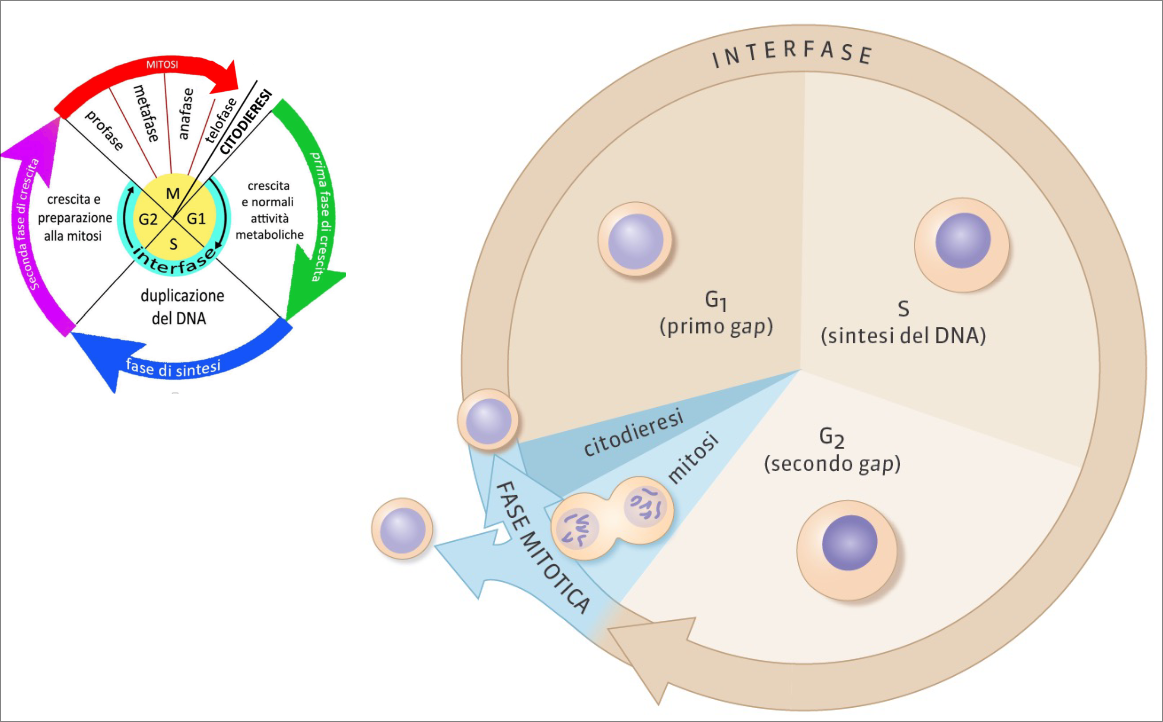
\includegraphics[width=\textwidth]{./resources/ciclo_cellulare}
    \end{figure}
    \end{center}
\end{snippet}

\begin{snippet}{ciclo-cellulare-expl1}
    Nella fase g1 la cellula non fa nulla e continuano la loro vita svolgendo le loro funzioni metaboliche. 
    Le cellule staminali o quelle che diventano gameti entrano nella fase S in cui il DNA viene duplicato. 
    Nella fase G2 la cellula si prepara alla divisione, e inizia a spiralizzare la cromatina. 
    Tutto ciò si chiama interfase.
    Nella fase mitotica la cellula viene divisa nella mitosi e quanto tutto è separato si taglia e si hanno due cellule separate, questa fase si chiama citodieresi.
\end{snippet}

\begin{snippet}{ciclo-cellulare-illustration2}
    \begin{center}
    \begin{figure}[ht]
        \centering
        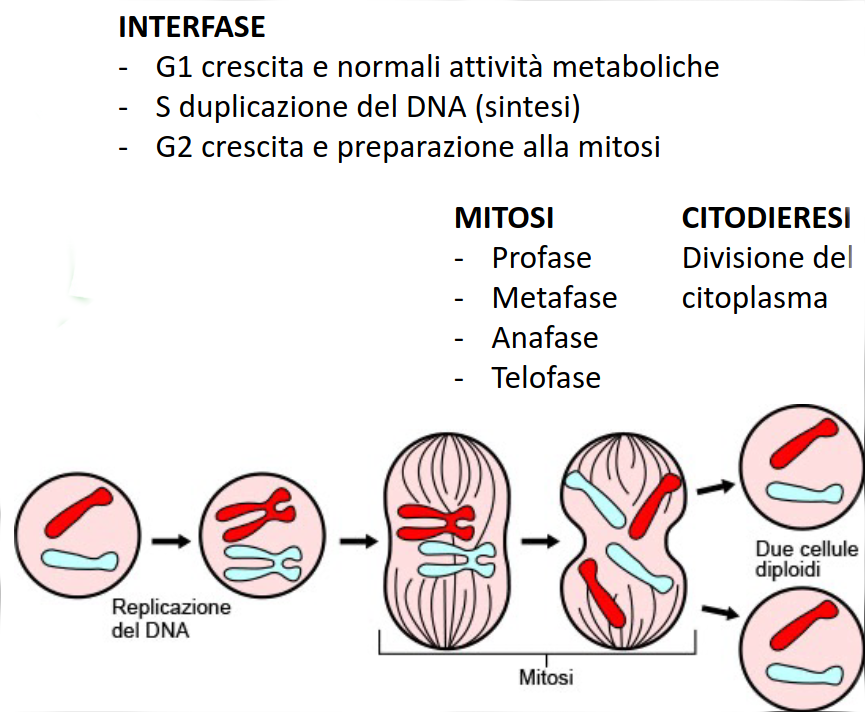
\includegraphics[width=0.6\textwidth]{./resources/ciclo_cellulare2}
    \end{figure}
    \end{center}
\end{snippet}

\begin{snippet}{ciclo-cellulare-expl2}
    Nella realtà la cromatina non contiene i cromosomi spiralizzati, a differenza del disegno.

    Il ciclo della cellula è controllato in base all'ambiente esterno.
    Se la cellula è sana e vi è nutrimento, la cellula può andare in mitosi.
    Vi sono quindi tre controlli o checkpoint che bloccano il passaggio ad una fase ulteriore
    se le condizioni non sono rispettate.
    Le cellule cancerogene eludono questi checkpoint.
\end{snippet}

\begin{snippet}{ciclo-cellulare-illustration3}
    \begin{center}
    \begin{figure}[ht]
        \centering
        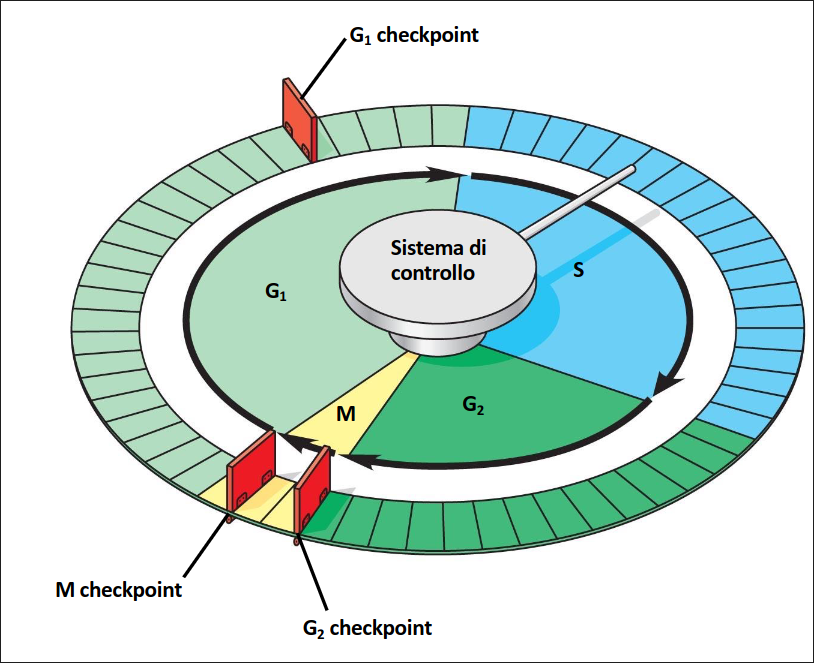
\includegraphics[width=0.75\textwidth]{./resources/ciclo_cellulare3}
    \end{figure}
    \end{center}
\end{snippet}

\begin{snippet}{ciclo-cellulare-expl2}
    Se la cellula diviene differneziata resterà sempre in G\({}_0\).
    \\
    Il DNA, durante tutta l'interfase, è sotto forma di cromatina nel nucleo.
    Durante la fase S dell'interface, inizia la duplicazione.
    Si creano delle bolle di duplicazione sui cromosomi, formando
    coppie di cromosomi omologhi duplicati (I cromosomi omologhi sono incollati fra di loro).
    Ogni cromosoma duplicato ha due cromatidi fratelli che sono assolutamente identici.
    In mitosi abbiamo solo a che vedere con cromosomi spiralizzati.
    I due cromatidi fratelli, appena staccati, diventano cromosomi e si posizionano in cellule diverse.

    Prima della meiosi e mitosi, vi è la medesima situazione: 46 cromosomi omologhi duplicati.
    Nella metafase della mitosi, i 46 cromosomi sono uno in fila all'altro,
    mentre nella meiosi si mettono a coppie uno in fila all'altro (per cui 23 coppie in fila).
\end{snippet}

\begin{snippetdefinition}{tetrade-definizione}{Tetrade}
    Nella metafase della meiosi, le coppie di cromosomi omologhi vengono chiamate
    \textit{tetradi}.
\end{snippetdefinition}

\begin{snippet}{meiosi-schema-illustration3}
    \begin{center}
    \begin{figure}[ht]
        \centering
        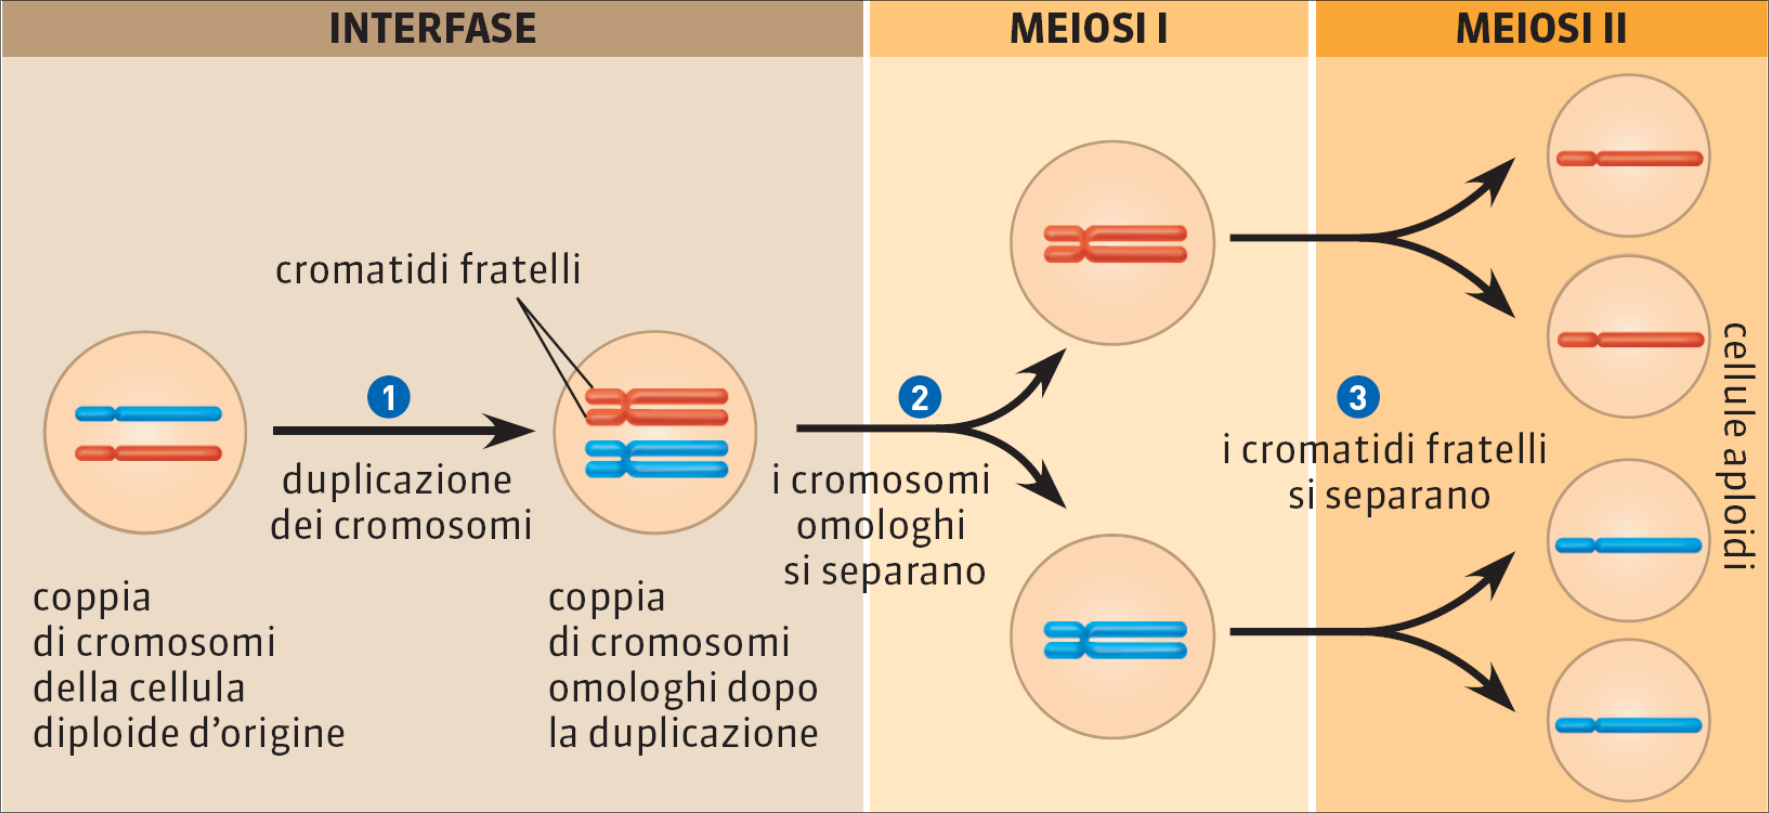
\includegraphics[width=0.75\textwidth]{./resources/meiosi_schema}
    \end{figure}
    \end{center}
\end{snippet}

% Schema MITOSI / MEIOSI giallo e violaceo
% Importantissimo da sapere tutto esattamente!!
% Meglio "duplicazione del materiale genetico" al posto di "duplicazione dei cromosomi"

\plain{I tumori hanno origine da mitosi mal riuscite.}

\section{Problemi della mitosi}

\begin{snippetdefinition}{trisomia-21-definizione}{Trisomia 21}
    La \textit{trisomia 21} è un disturbo per quale vi è un cromosoma extra (il cromosoma 21).
\end{snippetdefinition}

\begin{snippet}{trisomia21-illustration3}
    \begin{center}
    \begin{figure}[ht]
        \centering
        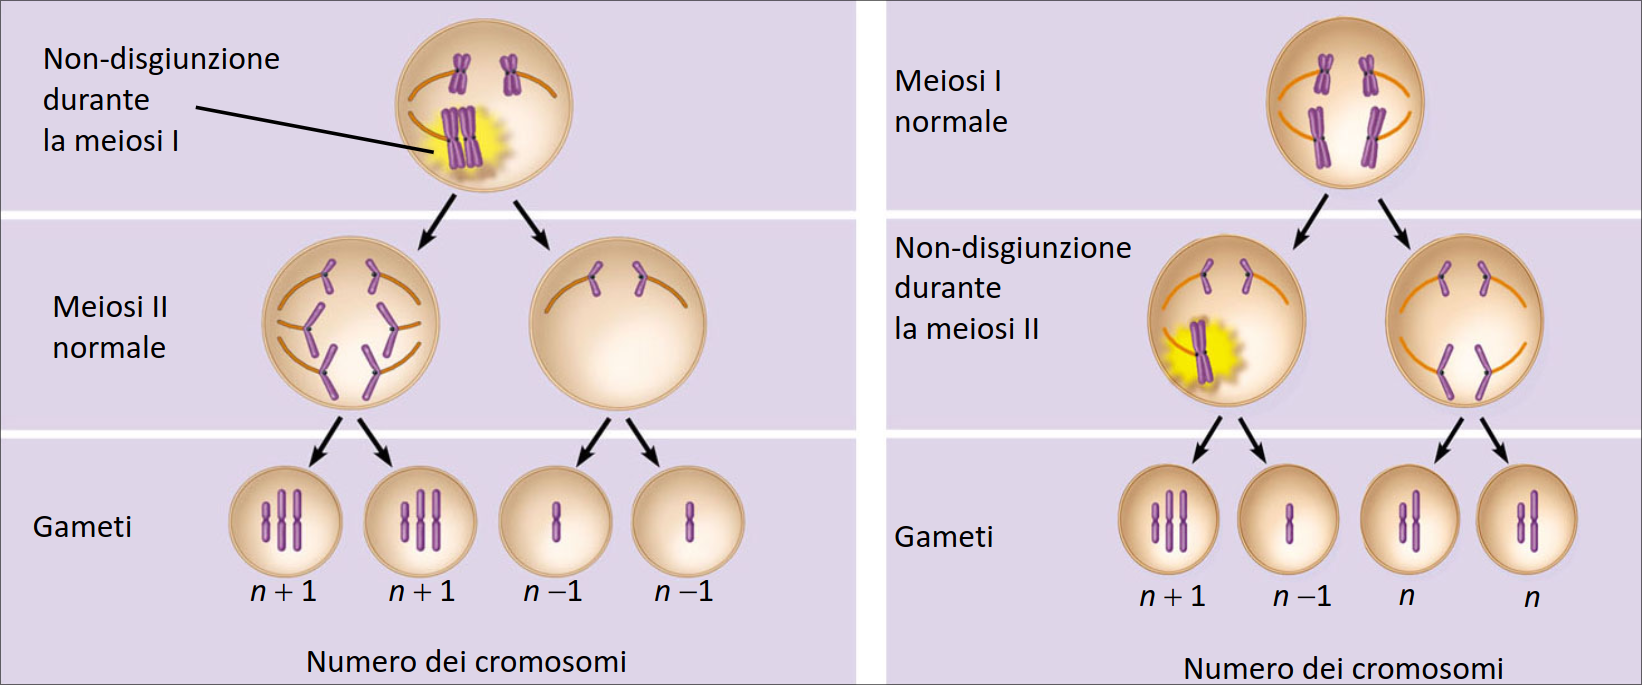
\includegraphics[width=0.75\textwidth]{./resources/trisomia21}
    \end{figure}
    \end{center}
\end{snippet}

\begin{snippet}{e924d64e-f74d-41d0-8a44-01ea950d6324}
    % TODO spiegare lo schema
    La motivazione più comune è data dalla madre, dove l'indice di rischio aumenta
    esponenzialmente dopo i 35 anni.
    Usando ovuli vecchi (gli ovuli sono prodotti alla nascita e rimangono gli stessi),
    è più probabile che i cromosomi non si stacchino.
\end{snippet}

\section{Problemi della meiosi}

\begin{snippet}{anomalie-meiosi-illustration3}
    \begin{center}
    \begin{figure}[ht]
        \centering
        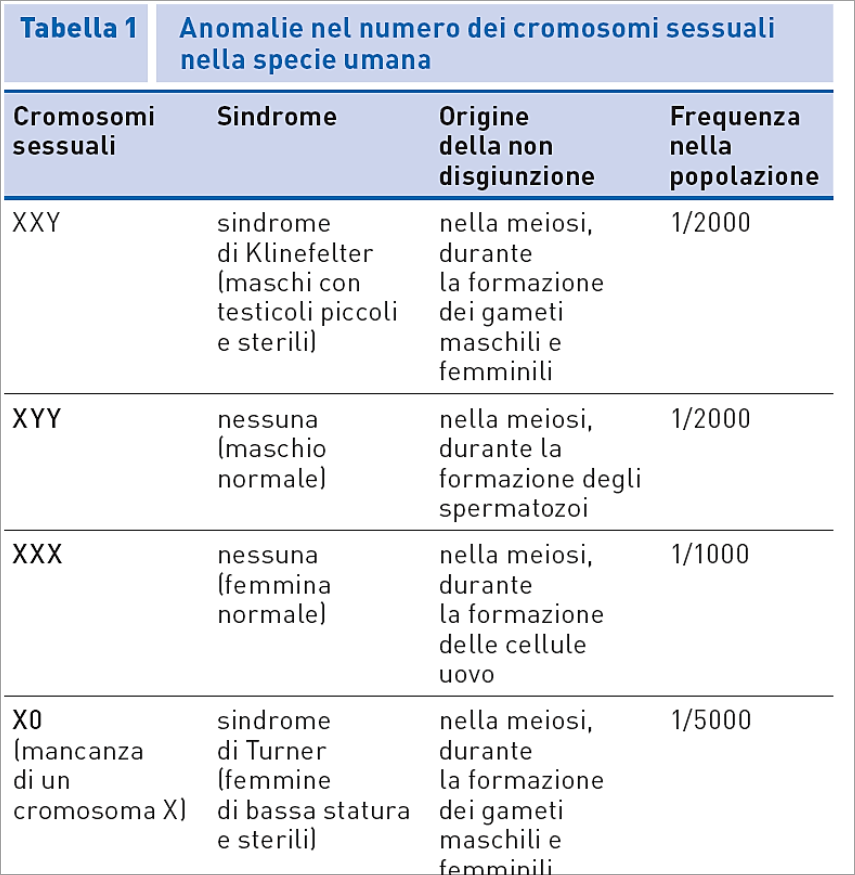
\includegraphics[width=0.75\textwidth]{./resources/anom}
    \end{figure}
    \end{center}
\end{snippet}

\begin{snippetdefinition}{sindrome-klinefelter-definizione}{Sindrome di Klinefelter}
    La \textit{sindrome di Klinefelter}
    è una trisomia XXY. Si tratta di uomini sterili con problemi dello sviluppo
    dei caratteri sessuali secondari:
    sterili, testicoli piccoli, pattern peli pubici femminile,
    pattern grasso pancia femminile, gynocomastia.
\end{snippetdefinition}

\begin{snippetdefinition}{sindrome-turner-definizione}{Sindrome di Turner}
    La \textit{sindrome di Turner} è
    una monosomia X0. Unicamente una delle due X funziona,
    mentre l'altra è in parte silenziata. Si tratta di femmine
    solitamente sterili con problemi dello sviluppo dei caratteri sessuali secondari.
\end{snippetdefinition}

\begin{snippet}{f982a995-039d-442d-8913-a5f95fad1e50}
    A volte possono capitare degli errori durnate la meiosi, che comportano:
    \begin{itemize}
        \item Alterazioni della \textbf{numero} dei cromosomi (\(\rightarrow\) mutazioni genomiche)
        \item Alterazioni nel \textbf{struttura} dei cromosomi (\(\rightarrow\) mutazioni cromosomiche)
    \end{itemize}
\end{snippet}

\end{document}